
\section{例子与图示}
\label{sec:examples-illustrations}

在第 2 章中我们从诸公理推得：$(\R^{2n},\omega_{0})$ 中的开球与柱体，对每个%
\trCapacity{}函数均有 $c\bigl(B(r)\bigr)=c\bigl(Z(r)\bigr)=\pi r^{2}$\footnote{原书右端印作「$e(Z(r))$」，径改「$c(Z(r))$」。——译者注}。这与%
$\partial B(r)$ 和 $\partial Z(r)$ 的诸\trClosedCharacteristic{}之\trAction{}相%
一致，正如我们在第 1 章中已经看到的那样。对一个椭球 $E$ 而言，\trCapacity{}%
$c(E)$ 也与 $\partial E$ 的某条特定\trClosedCharacteristic{}的\trAction{}相%
一致。回顾一下：$(\R^{2n},\omega_{0})$ 中一条\trLoop{} $\gamma$ 的（约化）%
\trAction{} $A(\gamma)$ 定义为
\[
A(\gamma)\ =\ \int_{\gamma}p\,dq\,.
\]

现在我们更一般地考察 $\R^{2n}$ 的一个\trConvex、\trBounded{}且\trSmooth{}的%
\trDomain{} $D$。正如我们在第 1 章中所证明的，它的\trBoundary{} $\partial D$%
上至少承载着一条\trClosedCharacteristic。结果表明，对上面所构造的特殊%
\trCapacity{}函数 $c_{0}$ 而言，$c_{0}(D)$ 同样由 $D$ 的\trBoundary{}的一条%
特定\trClosedCharacteristic{}所表示。

\begin{theorem}\label{thm:convex-domain-representation}
设 $C\subset\R^{2n}$ 是一个\trConvex\trBounded\trDomain，其\trBoundary{}%
$\partial C$ \trSmooth。于是存在一条特定\trClosedCharacteristic{}%
$\gamma^{*}\subset\partial C$，满足
\[
c_{0}(C,\omega_{0})\ =\ \bigl|A(\gamma^{*})\bigr|
\]
以及
\[
\bigl|A(\gamma^{*})\bigr|\ =\ \inf\Bigl\{\,\bigl|A(\gamma)\bigr|\ :\ \gamma\subset\partial C\ \text{是一条\trClosedCharacteristic}\Bigr\}\,.
\]
\end{theorem}

\noindent\begin{minipage}{\linewidth}
\centering
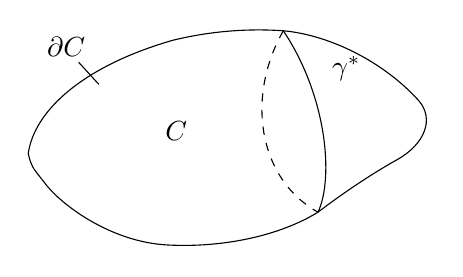
\begin{tikzpicture}[>=stealth,scale=0.8]
  \draw (0.7,2.5)
    .. controls (0.8,3.2) and (1.6,3.9) .. (3.0,4.3)
    .. controls (3.7,4.47) and (4.3,4.48) .. (4.75,4.45)
    .. controls (5.5,4.38) and (6.35,3.95) .. (6.9,3.34)
    .. controls (7.15,3.05) and (7.0,2.65) .. (6.55,2.4)
    .. controls (6.1,2.15) and (5.6,1.8) .. (5.3,1.57)
    .. controls (4.7,1.2) and (3.8,1.0) .. (2.9,1.05)
    .. controls (2.0,1.1) and (1.2,1.7) .. (0.95,2.05)
    .. controls (0.75,2.3) .. (0.7,2.5) -- cycle;
  \draw[dashed] (4.75,4.45) .. controls (4.15,3.4) and (4.35,2.1) .. (5.3,1.57);
  \draw (4.75,4.45) .. controls (5.45,3.4) and (5.55,2.1) .. (5.3,1.57);
  \node at (1.3,4.2) {$\partial C$};
  \draw (1.5,3.95) -- (1.82,3.6);%
  \node at (3.05,2.85) {$C$};
  \node at (5.75,3.85) {$\gamma^{*}$};
\end{tikzpicture}

图 3.8
\end{minipage}

本定理的证明与\cref{thm:z1-period-1}的证明颇为相似，我们请读者参阅%
H.~\trHofer{}与 E.~\trZehnder{}的文献 [123]。有一个%
有益的事实值得指出：同样的表示公式对那个定义在 $\R^{2n}$ 的子集上、原本由 I.~\trEkeland{}%
与 H.~\trHofer{}在 [68] 中引入的另一个\trCapacity{}函数也成立。从而，这两个%
\trCapacity{}在这类\trConvex{}子集 $C\subset\R^{2n}$ 上是一致的。作为另一个%
直接的推论，我们得出：对\trConvex、\trCompact{}且\trSmooth{}的\trHypersurface{}%
$\partial C$ 上的诸\trPeriodicSolution{} $x$ 的\trAction{}而言，下述%
\trEstimate{}成立：
\[
\bigl|A(x)\bigr|\ \geq\ \sup\Bigl\{\ \pi r^{2}\ \Bigm|\ \text{存在一个\trSymplecticEmbedding}\ \ \varphi:B(r)\to C\Bigr\}\ =\ D(C,\omega_{0})\,.
\]
这里我们用到了 $c_{0}$ 的\trMonotonicity。这个\trEstimate{}大幅锐化了%
C.~\trCroke{}与 A.~\trWeinstein{}在 [58] 中关于\trConvex\trHypersurface{}的%
\trPeriodicSolution{}的一个不等式。A.~\trKunzle{} [131] 观察到，%
\cref{thm:convex-domain-representation}还可用来描述 $\R^{2n}$ 中一类简单的%
\trCompact\trHypersurface，它们无法借助\trSymplecticDiffeomorphism{}被映射成%
\trConvex\trHypersurface。考察 $\R^{2n}$ 中一个具有\trSmooth{}\trBoundary{}%
$S=\partial M$ 的开的有界\trDomain{} $M$，满足
\[
B(r)\ \subset\ M\ \subset\ Z(r)
\]
它是一个满的\textbf{波尔多酒瓶}（Bordeaux bottle），如下图所示：

\noindent\begin{minipage}{\linewidth}
\centering
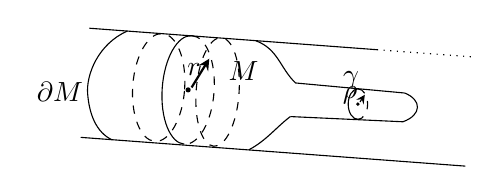
\begin{tikzpicture}[>=stealth,scale=0.44]
  \draw (1.45,5.05) -- (9.75,4.43);
  \draw[dotted] (9.75,4.43) -- (12.55,4.22);
  \draw (1.2,1.9) -- (12.3,1.07);
  \draw (2.55,4.97) .. controls (1.7,4.6) and (1.35,3.7) .. (1.4,3.15)
        .. controls (1.45,2.55) and (1.65,2.05) .. (2.1,1.83);
  \begin{scope}[rotate around={-4:(3.45,3.34)}]
    \draw[dashed] (3.45,3.34) ellipse [x radius=0.75, y radius=1.56];
  \end{scope}
  \begin{scope}[rotate around={-4:(4.3,3.27)}]
    \draw (4.3,4.84) arc[start angle=90, end angle=270, x radius=0.75, y radius=1.57];%
    \draw[dashed] (4.3,4.84) arc[start angle=90, end angle=-90, x radius=0.75, y radius=1.57];%
  \end{scope}
  \begin{scope}[rotate around={-4:(5.15,3.21)}]
    \draw[dashed] (5.15,3.21) ellipse [x radius=0.62, y radius=1.57];
  \end{scope}
  \fill (4.3,3.27) circle (0.075);
  \draw[->,thick] (4.4,3.34) -- (4.91,4.17);
  \node at (4.47,3.85) {$r$};
  \draw (6.25,4.69) .. controls (6.9,4.45) and (6.95,3.9) .. (7.4,3.47)
        -- (10.55,3.18);
  \draw (10.55,3.18) .. controls (11.05,2.98) and (11.05,2.55) .. (10.5,2.35);
  \draw (7.25,2.5) -- (10.5,2.35);
  \draw (6.05,1.54) .. controls (6.55,1.8) and (6.85,2.2) .. (7.25,2.5);
  \draw (9.2,3.3) arc[start angle=90, end angle=270, x radius=0.28, y radius=0.44];%
  \draw[dashed] (9.2,3.3) arc[start angle=90, end angle=-90, x radius=0.28, y radius=0.44];%
  \fill (9.2,2.86) circle (0.055);
  \draw[->] (9.26,2.92) -- (9.4,3.13);
  \node at (8.97,3.12) {$\rho$};
  \node at (9.0,3.55) {$\gamma$};
  \node at (0.6,3.2) {$\partial M$};
  \node at (5.9,3.8) {$M$};
\end{tikzpicture}

图 3.9
\end{minipage}

特别地，$M$ 内含有一段半径 $\rho<r$ 的\trCylinder{} $Z(\rho)$。在这一段上，%
$\partial Z(\rho)$ 的诸特征 $\gamma$ 都是\trClosed{}的，并且具有\trAction{}%
$A(\gamma)=\pi\rho^{2}$。现在用反证法假设 $\varphi$ 是 $\R^{2n}$ 的一个把 $M$%
映满\trConvex\trDomain{} $C$ 的\trSymplecticDiffeomorphism。于是它把%
\trHypersurface{} $\partial M$ 映满\trConvex\trHypersurface{} $\partial C$。由%
\trCapacity{}函数的\trInvariance，我们推得
\[
\pi r^{2}\ =\ c_{0}(M)\ =\ c_{0}\bigl(\varphi(M)\bigr)\ =\ c_{0}(C)\,.
\]
于是由\cref{thm:convex-domain-representation}，对 $\partial C$ 的一切特征%
\trLoop{} $\gamma$ 都有 $A(\gamma)\geq\pi r^{2}$。但 $\varphi$ 保持\trAction{}%
不变，于是
\[
\pi\rho^{2}\ =\ A(\gamma)\ =\ A\bigl(\varphi(\gamma)\bigr)\ <\ \pi r^{2}\ \leq\ A\bigl(\varphi(\gamma)\bigr)
\]
这就导致了矛盾。显然，上述\trManifold{} $M$ 的\trCapacity{}同样由 $\partial M$%
上的一条\trClosedCharacteristic{}所表示，然而这条\trClosedCharacteristic{}并%
不使\trAction{}极小。至于一般的具有\trSmooth{}\trBoundary{}的\trDomain，这里应当%
记得：$\R^{2n}$ 中每个\trCompact\trHypersurface{}是否都拥有%
\trClosedCharacteristic，尚属未知。

在二维\trCompact\trSymplecticManifold{}的特殊情形，诸正则\trEnergySurface{}%
当然都是一维的，并且由有限多条\trPeriodicOrbit{}组成。这一观察使 K.F.~\trSiburg{}%
[194] 得以算出这种情形下的\trCapacity{} $c_{0}$：

\begin{theorem}[K.F.~\trSiburg]\label{thm:siburg-c0-dim2}
设 $(M,\omega)$ 是一个\trCompact{}且\trConnected{}的\trSymplecticManifold，它%
可以带有\trBoundary，并设 $\dim M=2$。于是
\[
c_{0}(M,\omega)\ =\ \Bigl|\int_{M}\omega\Bigr|\,.
\]
\end{theorem}

我们看到 $c_{0}$ 与总体积相一致，从而在二维情形，这个\trInvariant{}便把诸%
\trSymplectic\trDiffeomorphic\trManifold{}分类。这已在第 1 章中证明。

\begin{proof}
我们先证明：对每个\trCapacity{}函数 $c$ 有
\[
c(M,\omega)\ \geq\ \Bigl|\int_{M}\omega\Bigr|\,.
\]
给定 $\varepsilon>0$。通过从 $M$ 上移去有限多条\trCompact\trCurve，我们便找到%
一个\trSimplyConnected{}的\trManifold{} $N\subset M$，它\trDiffeomorphic{}于一个%
\trClosed\trDisc{} $D\subset\R^{2}$，并且满足
\[
\Bigl|\int_{N}\omega\Bigr|\ \geq\ \Bigl|\int_{M}\omega\Bigr|-\varepsilon\,,
\]
而且我们可以选取\trDisc{} $D$ 的半径，使得它的\trLebesgue{}测度 $\mu(D)$ 与%
$\omega$ 在 $N$ 上的积分相一致。（回顾一下：黎曼曲面可以这样得到——取平面上%
的一个多边形并适当地粘合其各边；因此我们只须移去与这些边相对应的曲线便得到%
一个圆盘；参见 W.~\trMassey{}的文献 [148]。）依据\trDacorogna{}与\trMoser{}的定理（见%
第 1 章中的\cref{thm:dacorogna-moser}），这个\trDiffeomorphism{}可以被取成%
\trSymplectic{}的。于是，依据\trCapacity{}的\trMonotonicity，
\[
c(M,\omega)\ \geq\ c(N,\omega)\ =\ c(D)\ =\ \mu(D)\ \geq\ \Bigl|\int_{M}\omega\Bigr|-\varepsilon\,.
\]
这对每个 $\varepsilon>0$ 都成立，于是所要的\trEstimate{}得证。尚须证明
\[
c_{0}(M,\omega)\ \leq\ \Bigl|\int_{M}\omega\Bigr|\,.
\]
鉴于\trConformality，我们可以假定右端的积分是正的。我们取 $\varepsilon>0$，%
并在 $\mathcal{H}(M,\omega)$ 中取一个 $H$，满足
\[
m(H)\ \geq\ \int_{M}\omega+\varepsilon\,.
\]
我们必须建立 $M$ 上 $\dot{x}=X_H(x)$ 的周期满足 $0<T\leq1$ 的非常值%
$T$-\trPeriodicSolution{}的存在性。以 $R\subset[0,m(H)]$ 记 $H$ 的诸%
\trRegular{}值所成之集。由于诸\trCritical{}水平所成之集是\trCompact{}的，并且%
（依据\trSard{}定理）是\trLebesgue{}\trMeasureZero{}的，我们便可找到有限多个%
两两不相交的区间 $I_{j}=[a_{j},b_{j}]\subset R$，满足
\[
\sum_{j}\ \bigl(b_{j}-a_{j}\bigr)\ \geq\ m(H)-\frac{\varepsilon}{2}\ \geq\ \int_{M}\omega+\frac{\varepsilon}{2}\,.
\]
由 $\mathcal{H}(M,\omega)$ 的定义，在 $\partial M$ 近旁有 $H\equiv m(H)$。于是，%
若 $h\in R$，则 $H^{-1}(h)$ 由有限多个\trEmbedding{}的\trCircle{} $S^{1}\subset M$%
组成，其中每一条都恰好承载着 $X_H$ 的一个（非常值的）\trPeriodicSolution{}%
$\gamma(t,h)$。对每个 $j$，选出 $H^{-1}[a_{j},b_{j}]$ 的一个\trConnectedComponent{}%
并称之为 $A_{j}$。当 $h\in I_{j}$ 时，它被一个由诸\trPeriodicSolution{}组成的%
\trSmooth{}族 $\gamma(t,h)$ 一一（单层）地覆盖，这些\trPeriodicSolution{}的周期记作%
$T(h)>0$。定义\trDiffeomorphism{} $\varphi=\varphi_{j}$
\[
\varphi\,:\,(t,h)\ \mapsto\ \gamma(t,h)\ \in\ A_{j}\,,
\]
其中 $0\leq t<T(h)$ 且 $a_{j}\leq h\leq b_{j}$。我们断言：
\[
\varphi^{*}\omega\ =\ dt\wedge dh\,.
\]
的确，由于对一切 $t$ 有 $H\bigl(\gamma(t,h)\bigr)=h$，并以下标标记偏\trDerivative，%
我们便得出 $\omega(\gamma_{t},\gamma_{h})=dH\bigl(\gamma(t,h)\bigr)(\gamma_{h})=1$。%
于是，对 $\xi$, $\eta\in\R^{2}$ 可算得 $\varphi^{*}\omega(\xi,\eta)=\omega(d\varphi\,\xi,\,d\varphi\,\eta)=\omega\bigl(\xi_{1}\gamma_{t}+\xi_{2}\gamma_{h},\ \eta_{1}\gamma_{t}+\eta_{2}\gamma_{h}\bigr)=\xi_{1}\eta_{2}-\xi_{2}\eta_{1}=(dt\wedge dh)(\xi,\eta)$，%
断言得证。从而，
\[
\int_{A_{j}}\omega\ =\ \int_{\varphi^{-1}(A_{j})}\varphi^{*}\omega\ =\ \int_{a_{j}}^{b_{j}}T(h)\,dh\,.
\]
现在用反证法：假设对一切 $h\in R$ 都有 $T(h)>1$。于是
\[
\int_{M}\omega\ \geq\ \sum_{j}\ \int_{A_{j}}\omega\ >\ \sum_{j}\ \bigl(b_{j}-a_{j}\bigr)\ \geq\ \int_{M}\omega+\frac{\varepsilon}{2}\,,
\]
这里用到了对 $m(H)$ 的假设。这一矛盾表明：的确存在 $h\in R$ 与一条%
\trPeriodicSolution{} $\gamma(h)$，它位于某个 $A_{j}$ 中并且周期满足%
$0<T(h)\leq1$。依据 $c_{0}$ 的定义，所要的\trEstimate{}便随之而来，于是该%
定理的证明完成。
\end{proof}

为了说明这个定理，我们考察一个无\trBoundary{}的\trCompact{}二维\trManifold。%
在这种情形，证明表明：对每个满足 $\max H-\min H>\Bigl|\int_{M}\omega\Bigr|$\footnote{原书积分下标排印过小难辨，依定理 4 口径径归一为 $\int_{M}\omega$。——译者注} 的%
$H\in C^{2}(M,\R)$，\trHamiltonianVectorField{} $X_H$ 都拥有一个周期%
$0<T\leq1$ 的「快速」\trPeriodicSolution。关于 $\R^{2}$ 的子集这一特殊情形，%
我们还愿意补充另一个初等的观察。我们从第 2 章知道：对每个\trCapacity{}函数%
而言，对 $\R^{2}$ 中具有\trSmooth{}\trBoundary{}的\trBounded\trConnected{}子集%
$D$ 都有 $c(D)=\operatorname{area}(D)$。由于特殊\trCapacity{} $c_{0}$ 还额外%
具有\trInnerRegularity，我们可以轻松地把这个命题推广到 $\R^{2}$ 的%
开子集上。

\begin{proposition}\label{prop:c0-area-open-planar}
若 $\Omega\subset\R^{2}$ 是一个开的有界且\trPathConnected{}的集合，则%
$c_{0}(\Omega,\omega_{0})=\operatorname{area}(\Omega)$。
\end{proposition}

\begin{proof}
用\trCompact{}集 $K_{j}\subset\mathring{K}_{j+1}$（$j\geq1$）穷竭%
$\Omega=\bigcup K_{j}$，并如下定义\trSmooth{}函数 $\beta_{j}:\Omega\to\R$：当%
$x\in K_{j}$ 时令 $\beta_{j}(x)=0$，当 $x\in\Omega\backslash K_{j+1}$ 时令%
$\beta_{j}(x)=1$。再定义 $\beta\in C^{\infty}(\Omega)$ 为
\[
\beta(x)\ =\ \sum_{j\geq1}\ \beta_{j}(x)\ ,\qquad x\in\Omega\,.
\]
于是当 $x\to\R^{2}\backslash\Omega$ 时 $\beta(x)\to+\infty$。现在取由 $\beta$%
的诸\trRegular{}值组成的一列 $b_{n}\to\infty$，并考察具有\trSmooth{}\trBoundary{}%
的诸\trCompact\trSymplecticManifold{} $D_{j}=\beta^{-1}(-\infty,b_{j}]$。于是%
$\Omega=\bigcup D_{j}$（$j\geq1$）。由于 $c_{0}$ 具有\trInnerRegularity，%
我们便得出：当 $j\to\infty$ 时 $c_{0}(\Omega)=\lim\ c_{0}(D_{j})$。另一%
方面，由\trLebesgue{}测度的\trRegularity{}我们求得：当 $j\to\infty$ 时%
$\operatorname{area}(\Omega)=\lim\ \operatorname{area}(D_{j})$。由于我们已经%
知道 $c_{0}(D_{j})=\operatorname{area}(D_{j})$，该命题便得证。
\end{proof}

虽然\trInvariant{} $c_{0}$ 是借助特殊的\trPeriodicSolution{}来定义的，但在二维%
情形它与面积紧密相关却一点也不令人惊讶，因为\trSymplecticForm{}就是面积形式。%
相比之下，在更高维数下\trCapacity{} $c_{0}$ 还未被理解。事实证明，计算这个%
\trCapacity{}极为困难。不过已有一些已知的例子，下面即将提到。

\begin{theorem}\label{thm:cpn-capacity}
考察 $(\C P^{n},\omega)$，其\trSymplecticStructure{}为与\textbf{\trFubiniStudyMetric}%
（Fubini-Study metric）相关联的那个标准结构。于是
\[
c_{0}(\C P^{n},\omega)\ =\ \pi\,.
\]
\end{theorem}

这个结果归功于 H.~\trHofer{}与 C.~\trViterbo{} [122]。我们在此不给出证明，只%
指出：该证明分析了 $\C P^{n}$ 中诸\trHolomorphic\trSphere{}的结构，并且基于%
一阶\trElliptic{}系统的\trFredholm{}理论。现在设 $(M,\omega)$ 是任意一个无%
\trBoundary{}的\trCompact\trSymplecticManifold，并以 $\pi_{2}(M)$ 表示诸映射%
$u:S^{2}\to M$ 的\trHomotopy{}类。于是存在一个映射 $\pi_{2}(M)\to\R$：
\[
u\ \mapsto\ \langle\omega,u\rangle\ =\ \int_{S^{2}}u^{*}\omega\ \in\ \R\,.
\]
如下定义 $\alpha^{*}(M)\in\R\cup\{\infty\}$：
\[
\alpha^{*}(M)\ =\ \inf\Bigl\{\,\langle\omega,u\rangle\ \Bigm|\ u\in\pi_{2}(M)\quad\text{且}\quad\langle\omega,u\rangle>0\Bigr\}\,.
\]
此外，若 $\pi_{2}(M)=0$，则取 $\alpha^{*}=\infty$。于是，下述归功于%
A.~\trFloer{} -- H.~\trHofer{} -- C.~\trViterbo{} [88] 与 \trMa{} [146] 的结果成立。%

\begin{theorem}\label{thm:product-capacity}
考察\trSymplecticManifold{} $\bigl(M\times\R^{2n},\ \omega\oplus\omega_{0}\bigr)$，%
其中 $n\geq1$，并设 $\alpha^{*}=\alpha^{*}(M)>0$ 或 $\alpha^{*}=\infty$。于是
\[
c_{0}\bigl(M\times B(r)\bigr)\ =\ c_{0}\bigl(M\times Z(r)\bigr)\ =\ \pi r^{2}\,,
\]
只要 $\pi r^{2}<\alpha^{*}$。
\end{theorem}

\trSymplectic\trTorus{} $T^{2n}$ 的情形将在下一章中讨论。

顺便指出，通过限制 $c_{0}(M,\omega)$ 的定义中所容许的\trHamiltonianFunction{}类，%
便能得到不同的\trCapacity{}函数。譬如，以 $\widetilde{\mathcal{H}}(M,\omega)$%
表示 $\mathcal{H}(M,\omega)$ 中使 $\nabla H$ 的\trSupport{}在 $M$ 中%
\trContractible{}的那些 $H$ 所成之类，并相应地令 $\widetilde{\mathcal{H}}_{a}%
(M,\omega)=\mathcal{H}_{a}(M,\omega)\cap\widetilde{\mathcal{H}}(M,\omega)$，则%
我们可以定义
\[
\tilde{c}_{0}\,(M,\omega)\ =\ \sup\ \Bigl\{\,m(H)\ \Bigm|\ H\in\widetilde{\mathcal{H}}_{a}(M,\omega)\Bigr\}\,.
\]
我们的证明表明 $\tilde{c}_{0}$ 是一个\trCapacity{}函数；与之相关联的诸%
\trPeriodicSolution{}都是\trContractible{}的。它显然满足
\[
D(M,\omega)\ \leq\ \tilde{c}_{0}\,(M,\omega)\ \leq\ c_{0}(M,\omega)
\]
其中 $D(M,\omega)$ 是第 1 章中引入的\trGromovWidth。
